\documentclass[a4paper, 10pt]{report}
\usepackage[italian]{babel}
\usepackage[T1]{fontenc}
\usepackage[utf8]{inputenc}
\usepackage{charter}
\usepackage{amsmath}
\usepackage{amsthm}
\usepackage{amsfonts}
\usepackage{graphicx}
\usepackage{wrapfig}
\usepackage{tcolorbox}
\usepackage{fancyhdr}
\usepackage{listings}
\usepackage{longtable}
\usepackage{multicol}
\usepackage{xcolor}

\usepackage{geometry}
\geometry{a4paper, left=2cm,right=2cm,top=2cm,bottom=2cm}

\pagestyle{fancy}
\lhead{}
\chead{}
\rhead{\bfseries 31 ottobre 2019 }
\lhead{\bfseries Segnali e immagini - laboratorio}

\newcounter{main}
\setcounter{main}{1}

\lstnewenvironment{code}[1][firstnumber=\themain,name=main]
  {\lstset{language=matlab,
           basicstyle=\medium\ttfamily,
           numbers=left,
           basicstyle=\small,
           columns=fullflexible,
           inputencoding=latin1,
           #1
          }
}
{\setcounter{main}{\value{lstnumber}}}


\begin{document}

\noindent \textbf{Esempio di stabilizzazione video:}

\begin{code}
%% Esercizio 5: video stabilizzazione
clear all
close all
load frames; % video preso da: https://www.youtube.com/watch?v=wHsrBJ4ynk4
%load frames_Phil 


for i=1:size(frames,4)        %scorro tutti i frame del video
    sub(:,:,:,i) = imresize(frames(:,:,:,i),1);  
    i
end
frames = sub;
clear sub;

[R,C,~,~] = size(frames);  %verifico quante righe e colonne ha il nuovo video per controllare che la resize non dia errori
figure; template = imcrop(frames(:,:,:,10));
template = rgb2gray(template);  %converto alla scala grayscale
[tR,tC] = size(template);  %prendo il numero di righe e di colonne di template (non conosco la dimensione in quanto preso col mouse)

% template_image = ones(R,C);
% template_image(round(R/2-tR/2):round(R/2+tR/2)-1,round(C/2-tC/2):round(C/2+tC/2)-1)=template;

figure;
for i=1:size(frames,4)
    comp  = frames(:,:,:,i);
    compg = rgb2gray(comp);
    cc = normxcorr2(template,compg);
    [max_cc, imax] = max((cc(:)));
    [ypeak, xpeak] = ind2sub(size(cc),imax(1)); %trasforma il singolo indice in coppie di incice  (capisco di quanto mi sono spostato)
    corr_offset = [(ypeak-size(comp,1)) (xpeak-size(comp,2))]; %calcola la traslazione necessaria a spostare il template sull'immagine
    new(:,:,:,i) = imtranslate(frames(:,:,:,i),[-(corr_offset(2)+round(C/2)), -(corr_offset(1) + round(R/2))],'FillValues',0); %fa in   
    %modo che il template sia al centro dell'immagine corrente
    ccs(:,:,i) = cc;
    
    subplot(221); imagesc(template); axis image; title('Template scelto');
    subplot(222); imagesc(compg); axis image;  title(strcat('Immagine originale: ', num2str(i)));
    subplot(223); imagesc(ccs(:,:,i)); colorbar; title('Mappa di cross-correlazione 2D');
    hold on;      scatter(xpeak, ypeak,'rX');
    subplot(224); imshow(new(:,:,:,i)); title('Immagine stabilizzata');
   
    %ref=new(:,:,:,i);
    i
    pause(0.5)
end

%trasforma le operazioni sopra in un video
vidObj = VideoWriter('stabilizedPhil.mp4');
open(vidObj);
figure;
for i=1:size(frames,4)
    subplot(121); imshow(frames(:,:,:,i));
    subplot(122); imshow(new(:,:,:,i));
    currFrame = getframe(gcf);
    writeVideo(vidObj,currFrame);
%     drawnow
    i
%      pause
end 
   close(vidObj);
\end{code}

\noindent \\Analisi codice:
\begin{longtable}{| p{.25\textwidth} | p{.70\textwidth} |}

\textbf{M = size(X,DIM)} & Ritorna la lunghezza della dimensione di X specificata dallo scalare DIM.

Nel caso di un video, le quattro dimensioni sono (righe, colonne, canali colore, n. frame).
\\\\
\textbf{B = imresize(A, SCALE)} & Ritorna l'immagine A riscalata in base a SCALA.
Se SCALE = 1 ritorna l'immagine originale; se SCALE = 0.5 ritorna limmagine ridotto della metà (== prende un pixel ogni due).
\\\\
\textbf{I2 = imcrop(I)} & Assegna ad I2 una sezione dell'immagine I. La sezione viene selezionata tramite mouse.
\\\\
\textbf{J = rgb2gray(I)} & Converte l'immagine da RGB a scala di grigi.
\\\\
\textbf{[I,J] = ind2sub(SIZE,INDEX)} & Converte INDEX in una coppia di indici (I, J) basandosi su una matrice di dimensione SIZE. 

Esempio:
\begin{center}
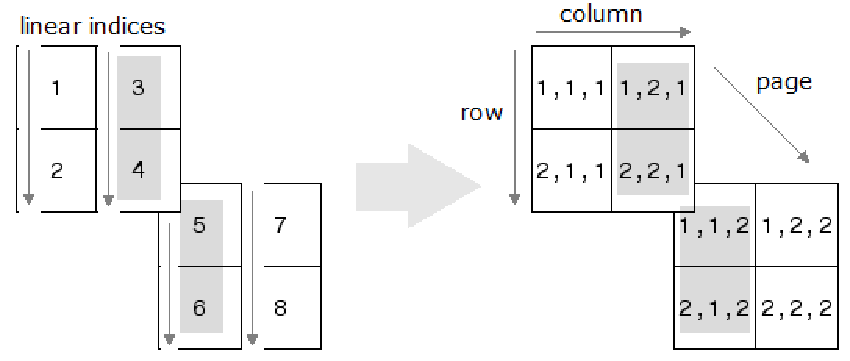
\includegraphics[scale=0.5]{ind2sub.pdf}

\lstset{language=matlab}
\begin{lstlisting}
ind = [3 4 5 6];
sz = [2 2 2];
[I1,I2,I3] = ind2sub(sz,ind)
\end{lstlisting}
\end{center}
\\\\\
\textbf{B = imtranslate(A,TRANSLATION)} & Trasla l'immagine A secondo il vettore TRANSLATION. Se A è 2D, il vettore è del tipo [x, y].
Il parametro 'FillValues' indica di che colore colorare gli spazi non più coperti dall'immagine.
\end{longtable}

\noindent Risultato:
\begin{center}
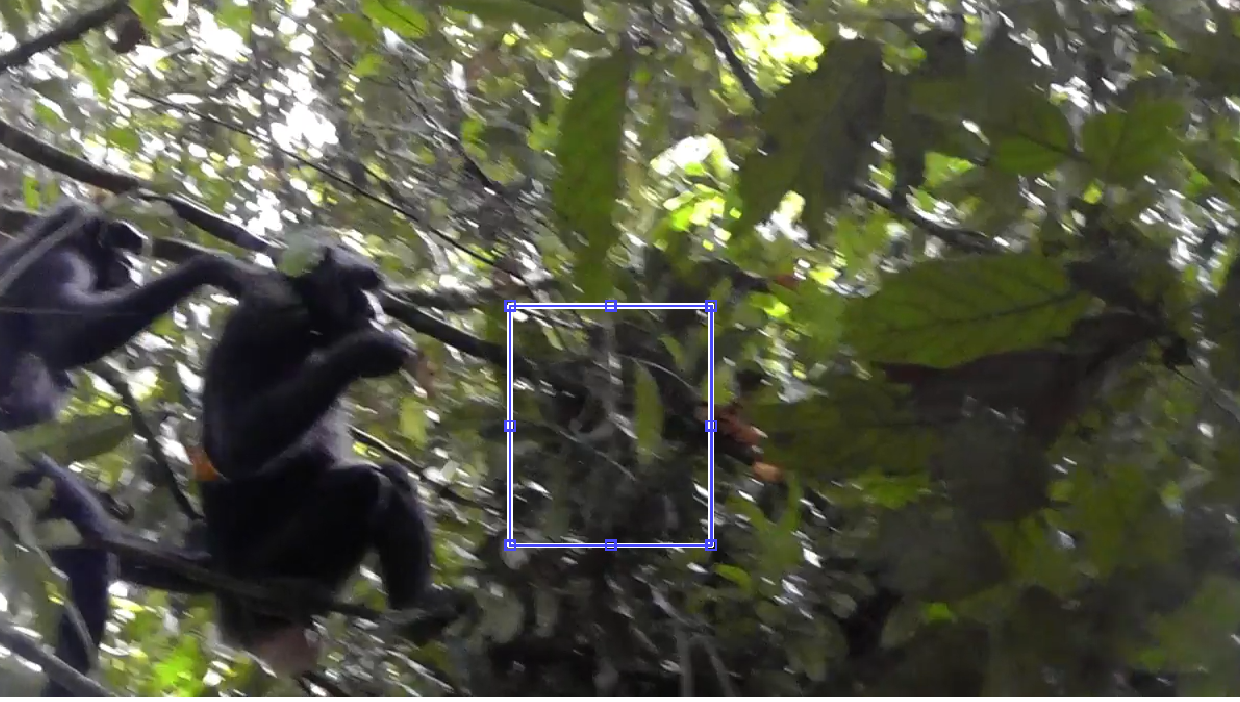
\includegraphics[scale=0.5]{base.pdf}

(Seleziono il template dal frame 10)

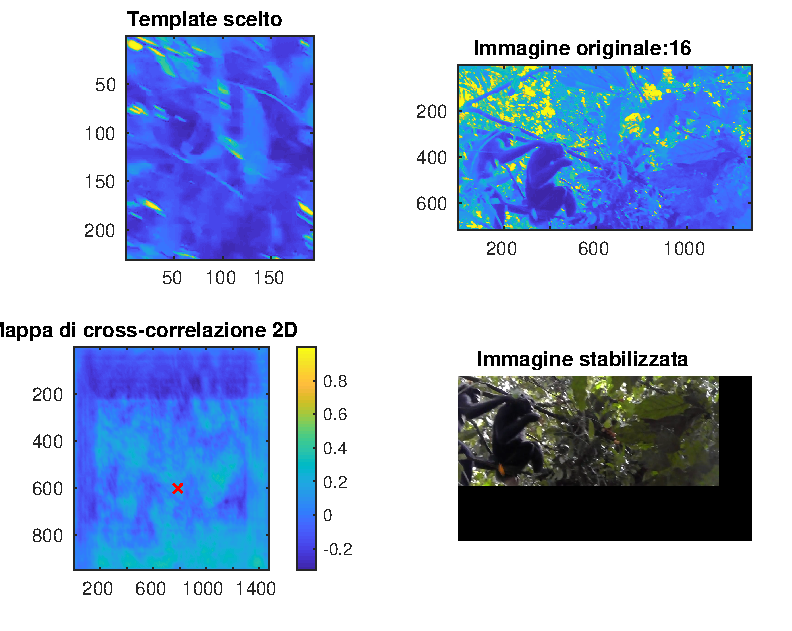
\includegraphics[scale=0.8]{2.pdf}

(Ripetizione per tutti e 61 i frame. Alla fine viene creato un video (non inserito))
\end{center}

\end{document}